% The \acrshort{soo} model for student-centred education is employed. 
% \Cref{fig:SOO} shows a graphical representation of all the subsequent activities of course material development using this model. 
% These activities are further described in the following sections.

% \begin{figure}[h]
%     \centering
%   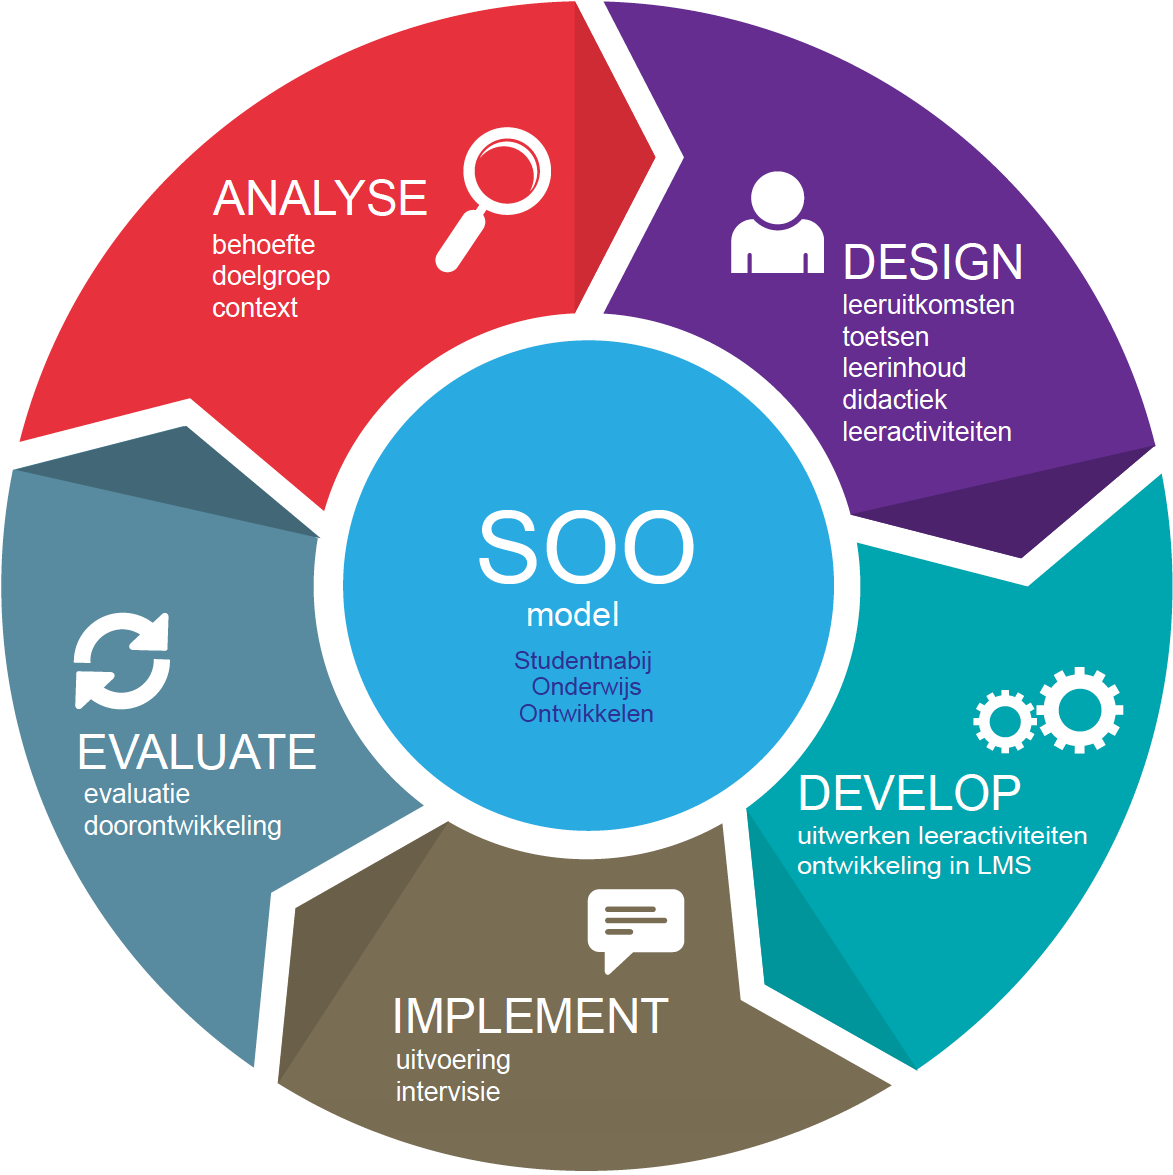
\includegraphics[width=0.5\textwidth]{figures/SOO_model.png}
%     \caption{Graphical representation of the \acrfull{soo} model (source: \url{https://portal.fhict.nl/medewerkersplein/Didactiek/Pages/Didactiek.aspx})}
%     \label{fig:SOO}
% \end{figure}


\subsection{Analyse}\label{chapter:didactics_phase_analyse}\label{chapter:didactics_phase_analyse}
Initially, the needs of students and the professional field are considered. My personal experience with \acrfull{pie} through student internships is in fact one of the reasons to develop a writing skills module. Generally, \acrshort{pie}'s feedback on written tasks boils down to \textit{informality in style }and difficulty to provide a \textit{smooth flow of ideas}. Furthermore, many alumni indicate struggles in the writing tasks, especially during the graduation. I am myself a \acrshort{fhict} alumna and I recognize similar lack of information.
\\\\
In my opinion, the most suitable audience for the writing skill module workshop are Semester 3 and Semester 6 students, respectively.
Both semester are in fact before the two internships, which are the two study unites heavily dependent on writing tasks. Furthermore, the students already acquire prior knowledge about the required content of the writing tasks within the project of ICT \& Software Engineering Semester 2, tasks which are repeated in the following semester, during a similar project involving \acrshort{pie}. Furthermore, additionally to the practice and experience of prior semesters, with Semester 6 the focus on research would increase, thus, so would the complexity of the the writing tasks.
\\\\
The writing module can be integrated in ICT \& Software Engineering Semester 3 as supportive workshop. While the development of Semester 6 is not yet started, I predict a similar context.
%Initially, a general picture of the course current situation was depicted, analyzing the \textit{target audience}, their \textit{needs} and the \textit{context} in which education is being developed. 
%Some example personas described in~\cref{appendices:personas} were composed to better understand the target audience.
%While the course is a fourth year elective, throughout my experience as an \acrshort{ale} teacher students that did not manage to find an internship project (thus, are half way in their third year) are usually joining electives to not waste an academic semester. 
%However, as a forth year ICT \& Software Engineering elective, \acrshort{ale} targets young professionals with a strong technical background, stimulated by applied mathematics and software engineering. 
%Preferably, \acrshort{ale} students should have studied in the ICT \& Software Engineering or ICT \& Technology profile and should have completed at least the first two academic years. For more details about the \acrshort{fhict} program see \cref{appendices:curriculum_structure}. 
%Furthermore, the needs of both the students and the professional field were considered, where solid software engineering competences were recognized essential, especially as an \acrshort{ict} graduate.
%Therefore, course material development would not imply changing the course structure, but \textit{clarify and enrich the learning experience}.
%As a consequence to the analysis, the context (such as instructional materials, learning environment) was realized and it is further described in the next section.

\subsection{Design}\label{chapter:didactics_phase_design}\label{chapter:didactics_phase_design}
\subsubsection{Learning outcomes}
For the writing skill module workshop I propose an additional learning outcome in each semester, namely communication in a written format.

\begin{figure*}[h!]
\begin{tabular}{|p{\textwidth}|}
 \hline
    \textbf{Learning outcome Semester 3: Basic communication writing skills}\\
    Communicate in a specific written task in the most appropriate manner.\\
 \hline
    \textit{Explanation}\\
    You use basic stylistic considerations and you are aware of your stylistic choices.
    \\ 
    You communicate information smoothly, using logical connections between ideas.\\
 \hline
\end{tabular}

\begin{tabular}{|p{\textwidth}|}
 \hline
    \textbf{Learning outcome Semester 6: Advanced communication writing skills}\\
    Communicate in a specific written task in the most appropriate manner.\\
 \hline
    \textit{Explanation}\\
    You use an appropriate/predictable format/pattern for a particular type of text (e.g. summary, introduction, data commentary).
    \\ 
 \hline
\end{tabular}
  \caption{Learning outcome for Semester 3 and Semester 6}
\end{figure*}

\begin{figure}[h!]
    \centering
   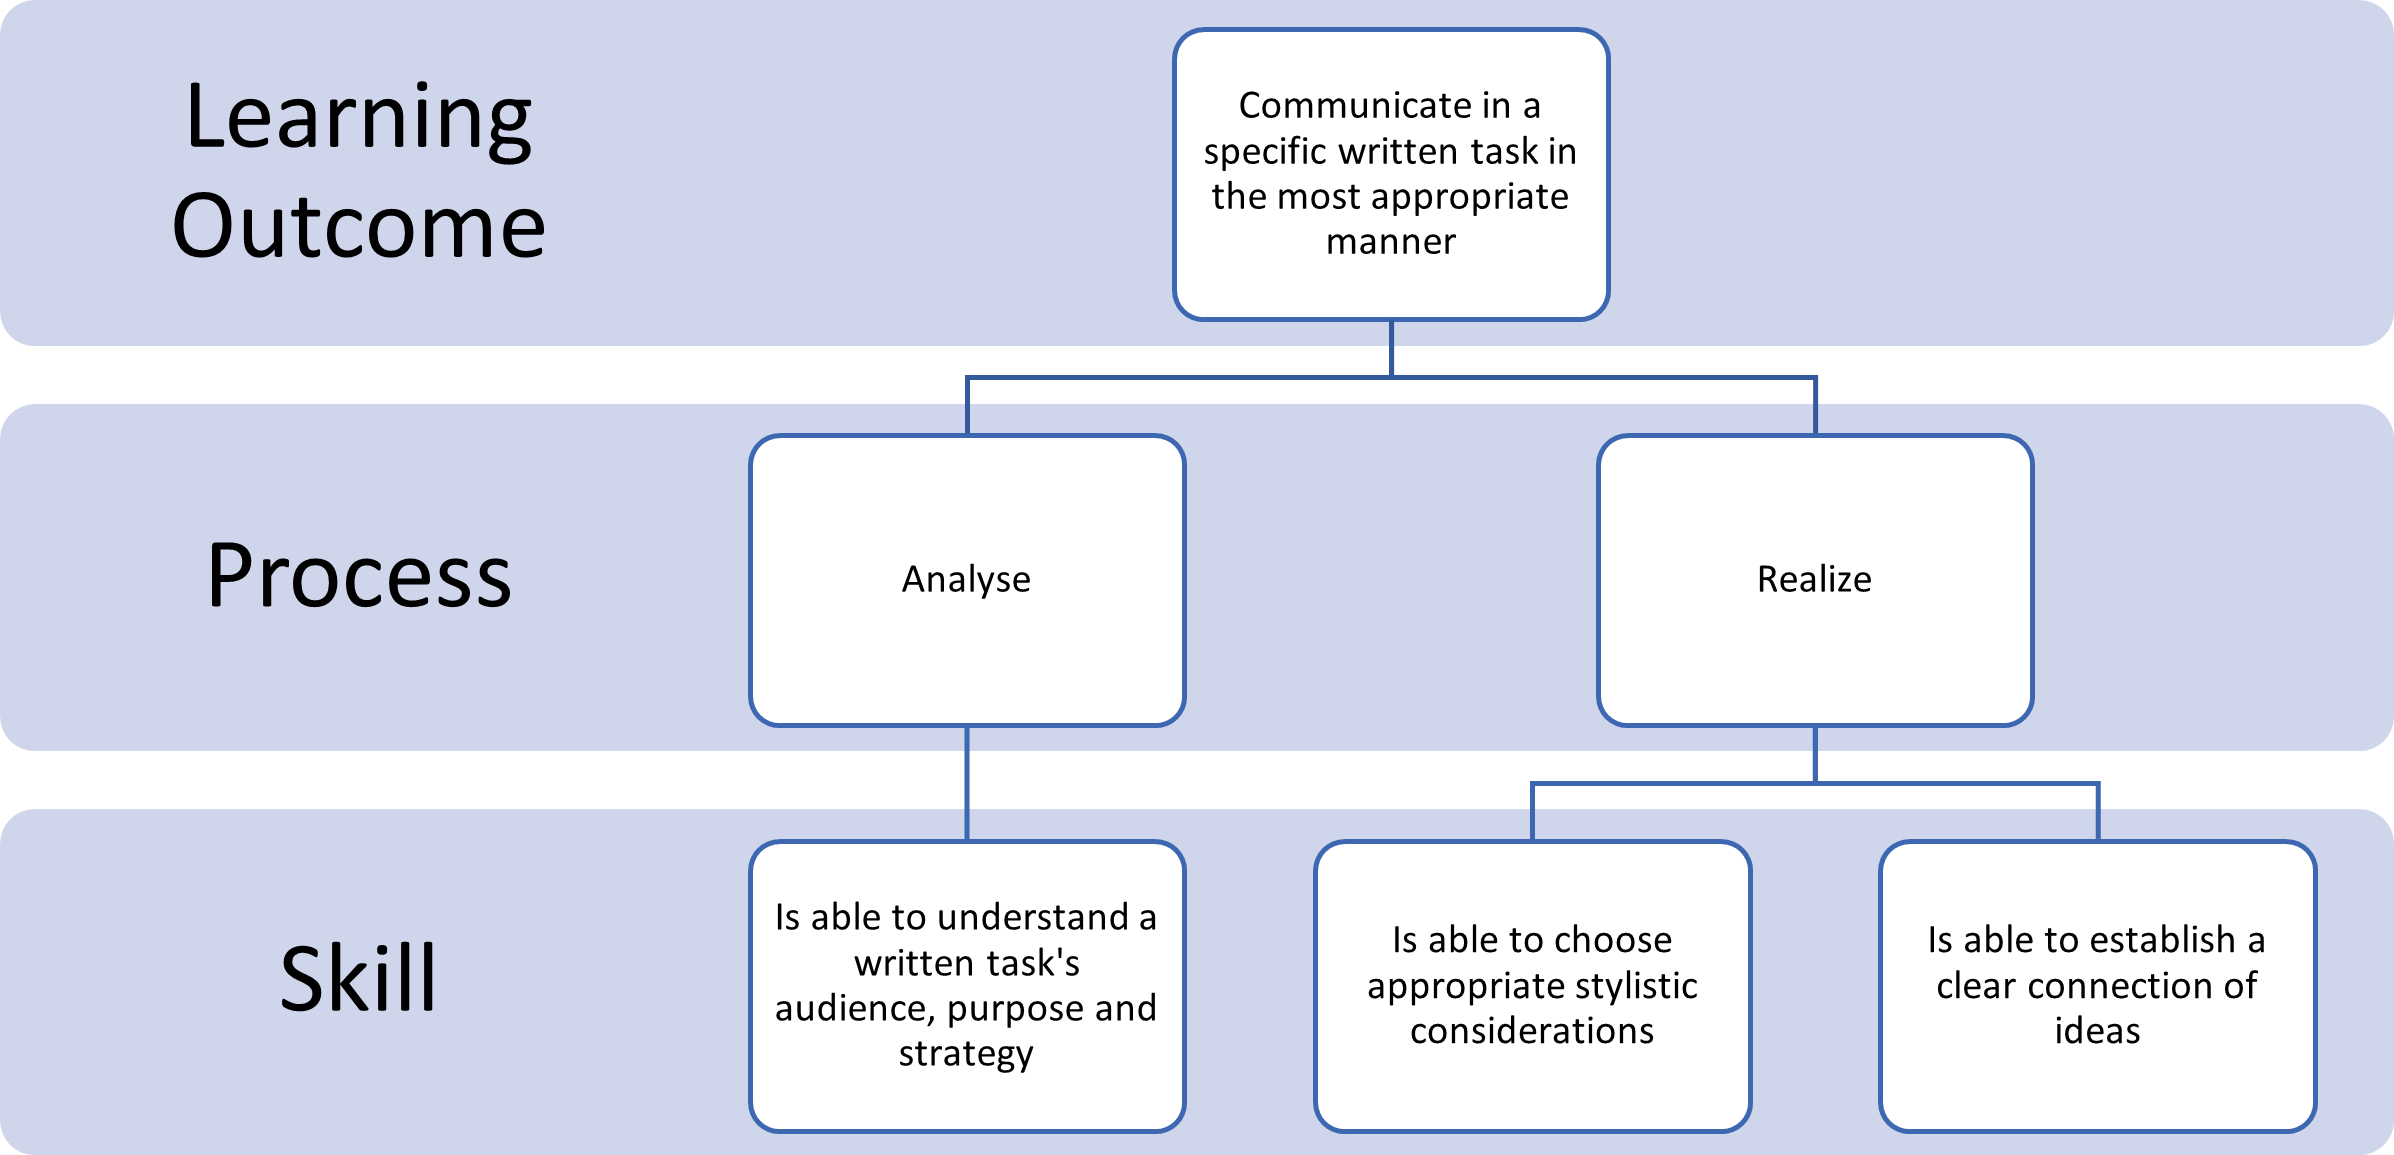
\includegraphics[width=\textwidth]{appendices/learning_outcomes/LO_S3.png}
    \caption{Skill tree for Semester 3 learning outcome: Basic communication writing skills}
    \label{fig:LO_S3}
\end{figure}

\begin{figure}[h!]
    \centering
   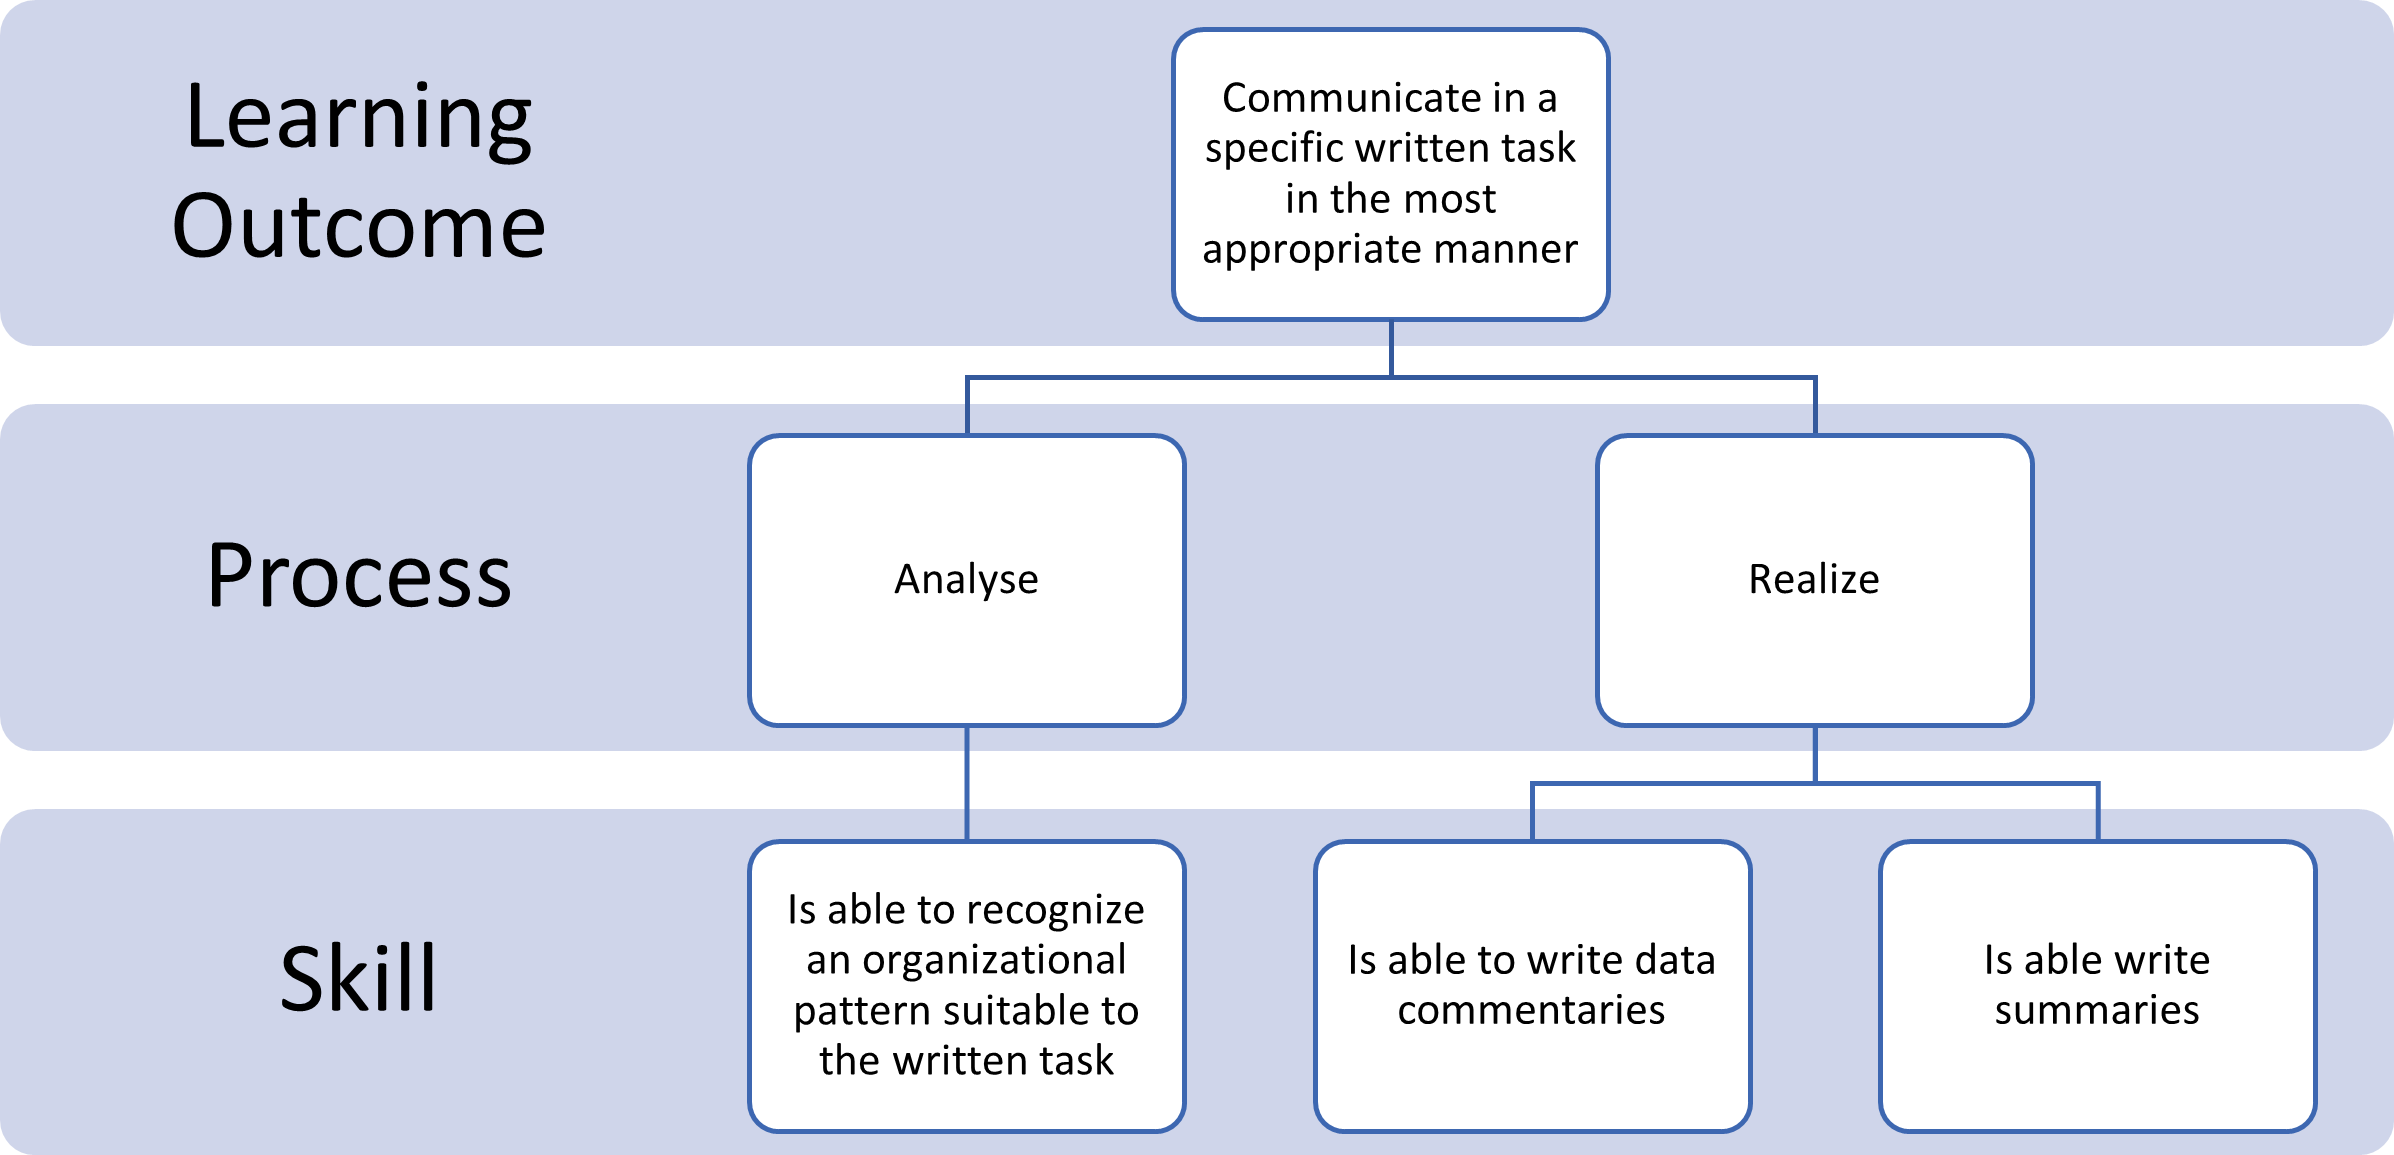
\includegraphics[width=\textwidth]{appendices/learning_outcomes/LO_S6.png}
    \caption{Skill tree for Semester 6 learning outcome: Advanced communication writing skills}
    \label{fig:LO_S6}
\end{figure}

\subsubsection{Learning activities}

The employed teaching method closely follows the \acrshort{4cid} model~\cite{FHICTTeachingMethods}. This model describes four basic components fitted to the course as follows:
\begin{itemize}
    \item learning tasks (weekly theory and practical lessons)
    \item supportive information (course notes and worked out examples, explanation of basics)
    \item practice tasks (individual tasks that aid to better understanding of topic)
    \item procedural information (feedback and feed forward through weekly individual short progress meetings)
\end{itemize}


\subsection{Develop}\label{chapter:didactics_phase_develop}\label{chapter:didactics_phase_develop}
Subsequently, the course material development followed. 
While original topics and assignments were preserved, only instructional materials were reworked.
Having rather considerable experience with the course subject, the task of developing lesson material suit me well. 
Furthermore, I have had the experience of fine-tuning instructional materials previously for other courses. The deliverables from this phase were:  
\begin{itemize}
    \item lesson slides
    \item assignment and supportive information (course notes)
    \item practice assignments
    \item \Gls{canvas} master course
\end{itemize}
While I could adapt and reuse former assignment examples, the majority is developed from scratch. 
I also added practice assignments (additional exercises) as a preparation for the assignment. 
Furthermore, example solutions of the assignments were constructed to aid future course teachers and reduce their preparation time.\\\\
A sample presentation along with the corresponding assignment and supportive information is provided in~\cref{appendices:slide_assignment_info}; this appendix includes also a sample solution and corresponding code snippet. 
An example of a \Gls{canvas} page is also attached in~\cref{appendices:slide_assignment_info}.\\\\
The most challenging task was to develop appropriate examples and practice assignments which would provide the basic understanding and would still require further self-engagement from the students.
Furthermore, researching trusted sources for further reading proved to be more time-consuming than expected. 
However, this experience has turned out to be quite enjoyable, and in the future I am looking forward to other development opportunities, even curriculum development.

\subsection{Implement}\label{chapter:didactics_phase_implement}\label{chapter:didactics_phase_implement}
The redesigned course material was first offered in the second half of the Fall semester 2020-2021, specifically for \acrshort{ale}2 which is about the automata topic. 
Due to the COVID-19 outbreak, within \acrshort{fhict} the lessons were \textit{blended}: online and face-to-face. In fact, according to a study by~\citet{blended2013}, the combination of blended learning produces stronger student learning outcomes than learning solely through face-to-face instruction. Another advantage of the online education is the possibility to record the theory parts of the lessons and make them available for revision. Further description of the use of technology during COVID-19 is given in~\cref{chapter:tel}.



\subsection{Evaluate}\label{chapter:didactics_phase_evaluate}\label{chapter:didactics_phase_evaluate}
To evaluate the effectiveness of the redeveloped course materials, the \acrshort{ale} Fall semester 2020-2021 students were first offered the old variant in \acrshort{ale}1, and the reworked variant in \acrshort{ale}2. Further description of the evaluation is presented in~\cref{chapter:research_expertise}. 
